%Vekt

\newcommand{\len}{\rg[Lengden av en vektor]{
		Lengden $ |\vec{u}|$ av en vektor $ {\vec{u}=[x_1, y_1, z_1]} $ er gitt som
		\nreq{|\vec{u}|=\sqrt{x_1^2+y_1^2+z_1^2} \label{lengd}} \vds
	}}
\newcommand{\lene}{\eks{
		Finn lengden av vektoren $ {\vec{u}=[-2, 4, 1]} $.
		
		\sv \vds
		\algv{
			|\vec{u}|&= \sqrt{(-2)^2+4^2+1^2} \\
			&= \sqrt{4+16+1} \\
			&= \sqrt{21}
		}\vds \vspace{-4pt}
	}}
\newcommand{\lvek}{
	\rg[Vektoren mellom to punkt]{
		Vektoren $ \vec{u} $ fra punkt $ {A=(x_1, y_1, z_1)}$ til ${B=(x_2, y_2, z_2) }$ er gitt som
		\begin{equation}\label{vektmpunkt}
		\vec{u}= [x_2-x_1, y_2-y_1, z_2-z_1] 
		\end{equation} \vds
	}}
\newcommand{\lveke}{\eks{
		Finn vektoren $ \vec{u} $ mellom punktet  ${A=(1, 2, 0) } $ og $ B=(3, 0,\\ 1) $.
		
		\sv \vds
		\algv{
			\vec{u} &= [3-1, 0-2, 1-0] \\
			& = [2, -2, 1]	}\vds
	}}
\newcommand{\skalen}{\rg[Skalarproduktet I]{
		Skalarproduktet av to vektorer  $ {\vec{u}=[x_1, y_1, z_1]} $ og $ {\vec{v}=[x_2, y_2, z_2]} $ kan skrives som	
		\begin{equation}
		\vec{u} \cdot \vec{v} = x_1 x_2+y_1 y_2+z_1 z_2
		\end{equation}
		
		For særtilfellet $ \vec{u}\cdot\vec{u} $ er
		\begin{equation}
		\vec{u}\cdot\vec{u}=\vec{u}^{\,2}
		\end{equation}	\vds
		
	}}
\newcommand{\skalene}{\eks{Finn skalarproduktet av vektorene $ {\vec{a}=[1, 2, 3]} $ og $ \vec{b}=[4,-3,\\-2] $.
		
\sv \vds
	\algv{\vec{a}\cdot\vec{b}&= 1\cdot4 + 2\cdot(-3)+3\cdot(-2)\\ &=-8 }\vds
	}}

\newcommand{\skalto}{\rg[Skalarproduktet II]{
		Skalarproduktet av to vektorer  $ \vec{u} $ og $ \vec{v}$ er gitt som
		\begin{equation}
		\vec{u} \cdot \vec{v}= |\vec{u}| |\vec{v}| \cos \theta \label{skal2}
		\end{equation}
		hvor $ \theta=\angle(\vec{u}, \vec{v}) $.
	} }
\newcommand{\skaltoe}{\eks[1]{
		En vektor $ \vec{a} $ har lengde 3 og en vektor $ \vec{b} $ har lengde 2. De utspenner vinkelen $ 45^\circ $. Finn skalarproduktet $ \vec{a}\cdot\vec{b}$. \\
		
		\sv
		\vs
		\vs
		\algv{\vec{a}\cdot\vec{b} &= 3\cdot2 \cos (45^\circ) \br
			&= 6\cdot\frac{\sqrt{2}}{2} \br
			&= 3\sqrt{2}}\vds
	}}
\newcommand{\skaltoeto}{\eks[2]{
		Finn vinkelen $ v$ utspent av vektorene $ {\vec{a}=[-5, 4, -3]}$ og $ {\vec{b}=[-2, 5, -5]} $. \\
		
		\sv
		Vi starter med å finne lengdene og skalarproduktene av vektorene:
		\alg{
			|\vec{a}|&= \sqrt{(-5)^2+4^2+(-3)^2} \\
			&= \sqrt{50} \\
			&= 5\sqrt{2} \\
			|\vec{b}| &= \sqrt{(-2)^2+5^2+(-5)^2} \\
			&= \sqrt{54} \\
			&= 3\sqrt{6} \\
			\vec{a}\cdot\vec{b} &= (-5)\cdot(-2) + 5\cdot4+(-3)\cdot(-5) \\&= 45
		}
		Videre har vi at
		\algv{\vec{a}\cdot \vec{b}&= |\vec{a}||\vec{b}|\cos v \\
			45 &= 5\sqrt{2}\cdot3\sqrt{6}\cos v \\
			\cos v &= \frac{5\cdot9}{5\cdot3\sqrt{12}} \\
			&= \frac{5\cdot9}{4\cdot3\cdot2\sqrt{3}}  \\
			&= \frac{3}{2\sqrt{3}} \\
			&= \frac{3}{2\sqrt{3}} \cdot \frac{\sqrt{3}}{\sqrt{3}} \\
			&= \frac{\sqrt{3}}{2}
		}
		Siden $ {\cos v = \frac{\sqrt{3}}{2}} $, er $ {v=30^\circ} $.
	}}
\newcommand{\vink}{\rg[Vinkelrette vektorer ]{
		To vektorer $ \vec{u} $ og $ \vec{v} $ står vinkelrett (normalt) på hverandre hvis skalarproduktet av dem er null:
		\begin{equation}\label{vnkr}
		\vec{u} \cdot \vec{v} = 0\iff \vec{u}\perp \vec{v}
		\end{equation}
		Hvis én av vilkårene i \eqref{vnkr} er oppfylt, sies $ \vec{u} $ og $ \vec{v} $ å være \textit{ortogonale}\index{ortogonal}.
	}}	
\newcommand{\para}{\rg[Parallelle vektorer]{
		To vektorer $ {\vec{u}=[x_1, y_1, z_1]} \text{ og } {\vec{v}=[x_2,y_2,z_2]} $ er parallelle hvis forholdet mellom korresponderende komponenter er likt
		\begin{equation}
		\frac{x_1}{x_2}=\frac{y_1}{y_2}=\frac{z_1}{z_2} \iff \vec{u}\parallel\vec{v}
		\end{equation}	\vs
	} }	
\newcommand{\parae}{\eks[1]{
		Gitt vektorene $ {\vec{u}=[1, 2, 3] }$ og ${\vec{v}=[3, 2(1-t), 11+t]} $, finn \textit{t} slik at $ \vec{u}$ og $ \vec{v} $ er parallelle.  \\
		
		\sv 
		Vi starter med å kreve at forholdet mellom korresponderende komponenter er likt. Vi dividerer $ x $- og $ y$-komponenten i $ \vec{v} $ med henholdsvis $ x $- og $ y$-komponenten i $ \vec{u} $:
		\begin{align*}
		\frac{3}{1} & = \frac{2(1-t)}{2} \\
		3 & = 1- t \\
		t &= -2
		\end{align*}
		Siden forholdet mellom de to $ x $-komponentene og de to $ y $-koordinatene er 3, må dette også stemme for $ z $-koordinatene for at $ \vec{u} $ og $ \vec v$ skal være parallelle:
		\begin{align*}
		\frac{11+t}{3} &= \frac{11+(-2)}{3} \\
		&= 3
		\end{align*}
		Altså er $ \vec{u}\parallel\vec{v} $ hvis ${ t=-2 }$.
	}}
\newcommand{\paraeto}{\eks[]{
		Et parallellogram er tegnet inn i figuren under.
		\begin{figure}
			\centering
			\includegraphics[]{\asym{par2}}
		\end{figure}
		Vis at midpunktet $ M $ til diagonalen $ AG $ også er midtpunktet til diagonalen $ CE $. \\
		
		\sv
		Vektoren $ \vv{AG} $ er gitt som
		\[ \vv{AG}= \vec{a}+\vec{b}+\vec{c} \]
		Dette betyr at
		\alg{
			\vv{AM}&= \frac{1}{2}\vv{AG} \\
			&= \frac{1}{2}(\vec{a}+\vec{b}+\vec{c}) 	
		}
		Vi kaller midpunktet til $ CE $ for $ M_1 $. Da har vi at
		\alg{
			\vv{CM_1} &= \frac{1}{2}\vv{CE}\\
			&= \frac{1}{2}(\vec{c}-\vec{a}-\vec{b})
		}
		Videre er
		\alg{
			\vv{AM_1}&=\vec{a}+\vec{b}+\vv{CM_1} \\
			&= \vec{a}+\vec{b}+ \frac{1}{2}(\vec{c}-\vec{a}-\vec{b})\\
			&= \frac{1}{2}(\vec{a}+\vec{b}+\vec{c}) \\
			&= \vv{AM}
		}
		Dette må bety at $ M=M_1 $.
	}}
\newcommand{\detto}{\rg[\boldmath$ 2\times 2 $ determinanter]{Determinanten $ \det(\vec{u}, \vec{v}) $ av to vektorer $ {\vec{u}=[a, b] }$ og $ {\vec{v}=[b, c]} $ er gitt som
		\algv{
			\det(\vec{u}, \vec{v}) &= \left|\begin{matrix}
				a & b \\
				c & d
			\end{matrix}\right| \\
			&= ad-bc	
		}\vds
	}}
\newcommand{\dettre}{\rg[\boldmath$ 3\times3$ determinanter]{
		Determinanten $ \det(\vec{u}, \vec{v}, \vec{w}) $ av tre vektorer $ {\vec{u}=[a, b, c]} $, $ {\vec{v}=[d, e, f]} $ og $ {\vec{w}=[g, h, i] }$ er gitt som
		\begin{align}
		\det(\vec{u}, \vec{v}, \vec{w}) &= \left|\begin{matrix}
		a & b & c \\
		d & e & f \\
		h & i & j
		\end{matrix}\right|\nonumber \\[5 pt]
		&= a\left|\begin{matrix}
		e & f \\
		i & j
		\end{matrix}\right|-b\left|\begin{matrix}
		d & f \\
		h & j
		\end{matrix}\right|+c\left|\begin{matrix}
		d & e \\
		h & i
		\end{matrix}\right| \label{3det1}
		\\[5 pt]
		&= a(ej-fi)-b(dj-fh)+c(di-eh) \label{3det2}
		\end{align}\vds
	}}
\newcommand{\dettree}{\eks{\label{eks33}
		Finn $ \det(\vec{a}, \vec{b}, \vec{c}) $ til vektorene $ \vec{a}=[1, -2, 2], \vec{b}=[2, 2, -3]  $ og \\ $ \vec{c}=[4, -1, 2] $.	\\
		
		\sv 
		Vi skal altså regne ut følgende:
		\[ 
		\left|\begin{matrix}
		1 & -2 & 2 \\
		2 & 2 & -3 \\
		4 & -1 & 2
		\end{matrix}\right|
		\]
		
		Å gå rundt å huske (\ref{3det2}) er ikke bare bare, så vi skal her bruke et triks som gjør det enklere for oss å komme fram til høyresiden i (\ref{3det1}).\vsk \\
		
		Vi starter med å finne tallet i første rad og kolonne, i vårt tilfelle 1. Deretter danner vi en $ {2\times 2}$ determinant ved å utelukke raden og kolonnen dette tallet tilhører:
		\begin{center}
			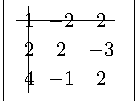
\includegraphics[]{fig/331}
		\end{center}
		Når vi ganger 1 med denne determinanten, har vi funnet det første leddet fra (\ref{3det1}):
		\[ 1\cdot\left|\begin{matrix}
		2 & -3  \\
		-1 & 2
		\end{matrix}\right| \]
		Vi går så over til tallet i første rad og andre kolonne, altså $ -2 $, og finner den tilhørende $ 2\times2 $ determinanten:
		\begin{center}
			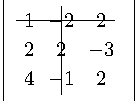
\includegraphics[]{fig/332}
		\end{center}
		Når vi setter et minustegn foran $ -2 $ ganger denne determinanten, har vi funnet andre ledd fra (\ref{3det1}):
		\[ -(-2)\cdot\left|\begin{matrix}
		2 & -3  \\
		4 & 2
		\end{matrix}\right| \]
		Vi avslutter med determinanten vi får ved å utelukke første rad og tredje kolonne:
		\begin{center}
			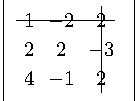
\includegraphics[]{fig/333}
		\end{center}
		Ganger vi denne med tallet som står i både raden og kolonnen som er utelatt, altså 2, får vi siste ledd i (\ref{3det1}):
		\[ 2\cdot\left|\begin{matrix}
		2 & 2  \\
		4 & -1
		\end{matrix}\right| \]
		Vi har nå funnet alle ledd vi trenger og kan da skrive
		\footnotesize
		\alg{
			\det(\vec{a}, \vec{b}, \vec{c}) &= 1\cdot\left|\begin{matrix}
				2 & -3  \\
				-1 & 2
			\end{matrix}\right|-(-2)\cdot\left|\begin{matrix}
			2 & -3  \\
			4 & 2
		\end{matrix}\right|+2\cdot\left|\begin{matrix}
		2 & 2  \\
		4 & -1
	\end{matrix}\right| \\
	&= 2\cdot2-(-3)\cdot(-1)+ 2(2\cdot2-(-3)\cdot4)+ 2(2\cdot(-1)-2\cdot4) \\
	&= 13
}\vds
}}
\newcommand{\detvo}{\rg[\boldmath$ 3\times3$ determinanter som volum]{Tallverdien til $\det(\vec{u}, \vec{v}, \vec{w})  $ tilsvarer volumet $ V $ av parallellepidetet utspent av $ \vec{u}, \vec{v}, \vec{w} $:
		\begin{equation}
		V = |\det(\vec{u}, \vec{v}, \vec{w})|
		\end{equation}		
	}}
\newcommand{\krypro}{\rg[Vektorproduktet]{
		Vektorpruduktet av vektorene $  {\vec{u}=[a, b, c]} $ og $ {\vec{v}=[d, e, f]} $ er gitt som
		\begin{equation}
		\vec{u}\times\vec{v}=[bf-ce, -(af-cd), ae-bd] \label{vekpro}
		\end{equation}
		Eventuelt kan man skrive
		\begin{equation}
		\vec{u}\times\vec{v} = \left|\begin{matrix}
		\vec{e}_x & \vec{e}_y & \vec{e}_z \\
		a & b & c \\
		d & e & f
		\end{matrix}\right| \label{vp1}
		\end{equation}
		hvor $ \vec{e}_x=[1, 0, 0], \vec{e}_y=[0, 1, 0] $ og $ \vec{e}_z=[0, 0, 1] $.\vsk
		
		Videre har vi at\footnote{Kryssprodukt må regnes ut før skalarprodukt}\vs
		\begin{align}
		&\vec{u}\times\vec{v}\cdot\vec{u}=0 \\
		&\vec{u}\times\vec{v}\cdot\vec{v} =0 \\
		&|\vec{u}\times\vec{v}|=|\vec{u}||\vec{v}|\sin \angle(\vec{u}, \vec{v}) \label{vekplen}
		\end{align}\vds\vs
	}}
\newcommand{\kryproe}{\eks{
		Regn ut vektorproduktet av vektorene $ {\vec{a}=[-3, 2, 3]} $ og $ {\vec{b}=[2, -2, 1]} $. \\
		
		\sv
		Vi bruker uttrykket fra (\ref{vp1})	og regner ut følgende $ {3\times3} $ determinant:
		\[ \vec{a}\times\vec{b} =\left|\begin{matrix}
		\vec{e}_x & \vec{e}_y & \vec{e}_z \\
		-3 & 2 & 3 \\
		2 & -2 & 1
		\end{matrix}\right|  \]
		Vi får da at (se gjerne tilbake til eksempelet på side \pageref{eks33})
		\small
		\alg{
			\vec{a}\times\vec{b}&=\vec{e}_x\left|\begin{matrix}
				2 & 3 \\
				-2 & -1
			\end{matrix}\right|-\vec{e}_y\left|\begin{matrix}
				-3 & 3 \\
				2 & 1
			\end{matrix}\right|+\vec{e}_z\left|\begin{matrix}
				-3 & 2 \\
				2 & -2
			\end{matrix}\right|  \\
			&= \vec{e}_x(2\cdot1-3\cdot(-2))-\vec{e}_y(-3\cdot1-3\cdot2)+\vec{e}_z(-3\cdot (-2)-2\cdot2) \\
			&= 8\vec{e}_x+9\vec{e}_y+2\vec{e}_z \\
			&= [8, 9, 2]	
		}\vds
	}}
\newcommand{\kryar}{\rg[Vektorproduktet som areal]{
	}}
\newcommand{\kryarvo}{\rg[Vektorproduktet som areal og volum]{
		Arealet $ A $ av et parallellogram utspent av vektorene $ \vec{u} $ og $ \vec{v} $ er gitt som
		\nreq{A = |\vec{u}\times\vec{v}| \label{vekpar} }
	%	\includegraphics[scale=1]{\asym{parll}}
		Arealet $ A $ av en trekant utspent av vektorene $ \vec{u} $ og $ \vec{v} $ er gitt som
		\nreq{A = \frac{1}{2}|\vec{u}\times\vec{v}|\label{vektre}}
		Volumet $ V $ av parallellepipedet utspent av vektorene $ \vec{u}$, $ \vec{v} $ og $ \vec{w} $ er gitt som
		\nreq{V = \left|\vec{u}\times\vec{v}\cdot\vec{w}\,\right|}
		%\includegraphics[scale=1]{\asym{par}}
		Volumet $ V $ av pyramiden utspent av vektorene $ \vec{u}$, $ \vec{v} $ og $ \vec{w} $ er gitt som
		\nreq{V = \frac{1}{3}|\vec{u}\times\vec{v}\cdot\vec{w}\,|\label{volavpyr} }
		%\includegraphics[scale=1]{\asym{pyram}}
		Volumet $ V $ til tetraedet utspent av vektorene $ \vec{u}$, $ \vec{v} $ og $ \vec{w} $ er gitt som			
		\nreq{ V = \frac{1}{6}|\vec{u}\times\vec{v}\cdot\vec{w}\,|}\vs
		%\includegraphics[scale=1]{\asym{tetra}}	
	}}
\newcommand{\rgnreg}{\rg[Regneregler for vektorer]{
		Gitt vektorene $ {\vec{u}=[x_1, y_1, z_1]} $ og $ {\vec{v}=[x_2, y_2, z_2]} $, punktet ${ A=(x_0,y_0,z_0)} $ og en konstant $ t $. Da er
		\begin{align}
		A+\vec{u} &= (x_0+x_1, y_0+y_1, z_0+z_1) \label{punktplvektor}	\\
		\vec{u}+\vec{v} &= [x_1+x_2, y_1+y_2, z_1+z_2] \\
		\vec{u}-\vec{v} &= [x_1-x_2, y_1-y_2, z_1-z_2] \\
		t\vec{u} &= [tx_1, ty_1, tz_1] \label{fellesfakt}
		\end{align}
		Figurativt kan vi tegne summen eller differansen av $ \vec{u} $ og $ \vec{v} $ som
		\begin{figure}
			\centering
			\subfloat[]{\includegraphics[scale=1]{\asym{uplusv}}}\qquad\quad
			\subfloat[]{\includegraphics[scale=1]{\asym{uminusv}}}
		\end{figure}\vs
		For en vektor $ \vec{w} $ har vi videre at
		\begin{align}
		(\vec{u}+\vec{v})+\vec{w} &= \vec{u}+(\vec{v}+\vec{w}) \\
		\vec{u}-(\vec{v}+\vec{w}) &= \vec{u}-\vec{v}-\vec{w}\\
		t(\vec{u}+\vec{v})&= t\vec{u}+t\vec{v}
		\end{align}\vds
}}
\newcommand{\kryproregn}{\rg[Regneregler for vektorproduktet]{
		For vektorene $ \vec{u}, \vec{v} $ og $ \vec{w} $ og en konstant $ t $ har vi at
		\begin{align}
		\vec{u}\times\vec{v} &= -\vec{v}\times\vec{u} \\
		\vec{u}\times{(t\vec{v})} &= t(\vec{u}\times\vec{v}) \\
		\vec{u}\times(\vec{v}+\vec{w})&=\vec{u}\times\vec{v}+\vec{u}\times\vec{w}\\
		\vec{u}\times\vec{v}\cdot\vec{w}&= \vec{w}\times\vec{u}\cdot\vec{v} \label{ukryvpriw}
		\end{align}\vds
}}
\newcommand{\skalrgn}{\rg[Regneregler for skalarproduktet]{
		For vektorene $ \vec{u} $, $ \vec{v} $ og $ \vec{w} $ har vi at
		\alg{
			\vec{u}\cdot\vec{v} &= \vec{v}\cdot\vec{u} \\
			\vec{u}\cdot\left(\vec{v}+\vec{w}\right) &= \vec{u}\cdot\vec{v}+\vec{u}\cdot\vec{w} \\
			\left(\vec{u}+\vec{v}\right)^2 &= \vec{u}^{\,2} + 2\vec{u}\cdot\vec{v}+\vec{v}^{\,2}
		}\vds
}}